\frame{

\begin{columns}

\column{.5\linewidth}

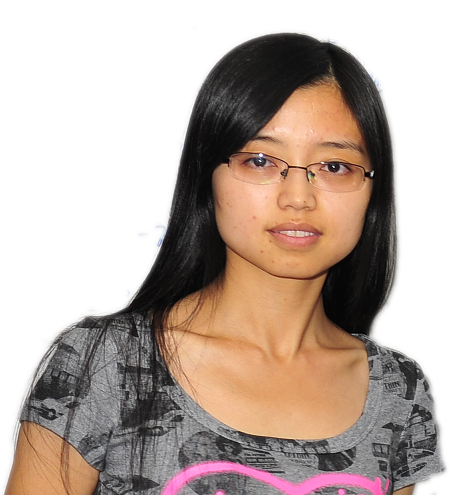
\includegraphics[width=.8\linewidth]{general_figures/yuening}

\column{.5\linewidth}

\begin{block}{Interactive Topic Modeling}
Yuening Hu, Jordan Boyd-Graber, and Brianna Satinoff.  Association for Computational Linguistics, 2011.
\end{block}

\end{columns}

}


\frame{

\frametitle{The Problem: User Perspective}

\begin{columns}

\column{.4\linewidth}
\begin{center}
\begin{tabular}{ccc}
& \only<2->{\itmspace}\color<2->{red}{bladder} & \\
& \only<3->{\hspace{-2cm}} \color<3->{blue}{spinal\_cord}  & \\
& \only<3->{\hspace{-2cm}} \color<3->{blue}{sci} & \\
& \only<3->{\hspace{-2cm}}\color<3->{blue}{spinal\_cord\_injury} & \\
& \only<3->{\hspace{-2cm}}\color<3->{blue}{spinal} & \\
& \only<2->{\itmspace}\color<2->{red}{urinary} & \\
& \only<2->{\itmspace}\color<2->{red}{urothelial} & \\
& \only<3->{\hspace{-2cm}}\color<3->{blue}{cervical} & \\
& injury & \\
& recovery & \\
& \only<2->{\itmspace}\color<2->{red}{urinary\_tract} & \\
& locomotor & \\
& \only<3->{\hspace{-2cm}}\color<3->{blue}{lumbar} & \\
\end{tabular}
\end{center}

\column{.6\linewidth}

\danquote{These words don't belong together!}

\end{columns}

}

\begin{frame}
        \frametitle{This is serious business!}


        \begin{itemize}
          \item Decision makers see problems
          \item No easy way to correct the problem
          \item Result: entire approach is abandoned
\pause
          \item Two ingredients in the fix:
            \begin{itemize}
              \item New models
              \item How to learn from mistakes
            \end{itemize}
        \end{itemize}

\end{frame}



\frame{
	\frametitle{Fix Ingredient \#1: The model}

\begin{columns}

\column{.4\linewidth}

\begin{itemize}
	\item The topics in a topic model are \only<2->{\alert<2>{uncorrelated}} distributions over words
	\only<3->{
	\item The advice you get can be encoded as correlations
		\begin{itemize}
			\alert<4>{\item Positive correlations}
			\alert<5>{\item Negative correlations}
		\end{itemize}
	}

\end{itemize}

\column{.6\linewidth}

	\only<1-2>{	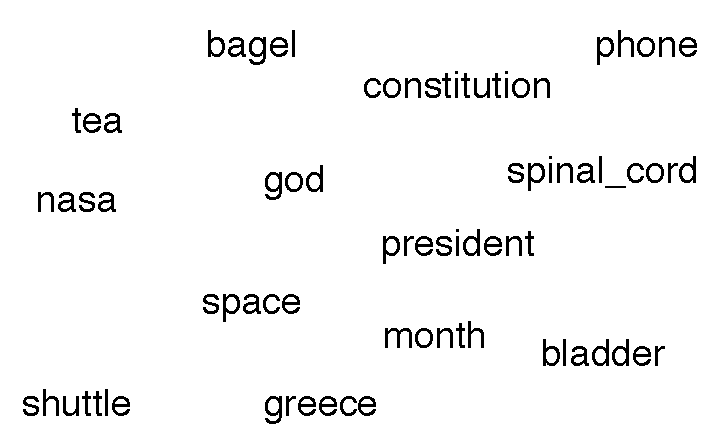
\includegraphics[width=\linewidth]{interactive_topic_models/constraints_1}     }
	\only<3-4>{	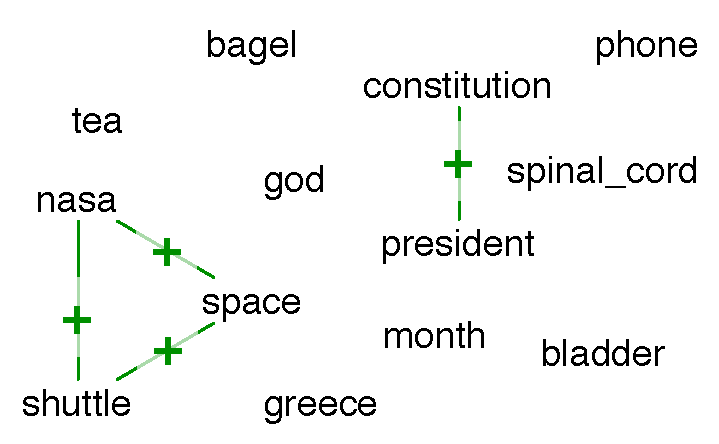
\includegraphics[width=\linewidth]{interactive_topic_models/constraints_2}     }
	\only<5->{	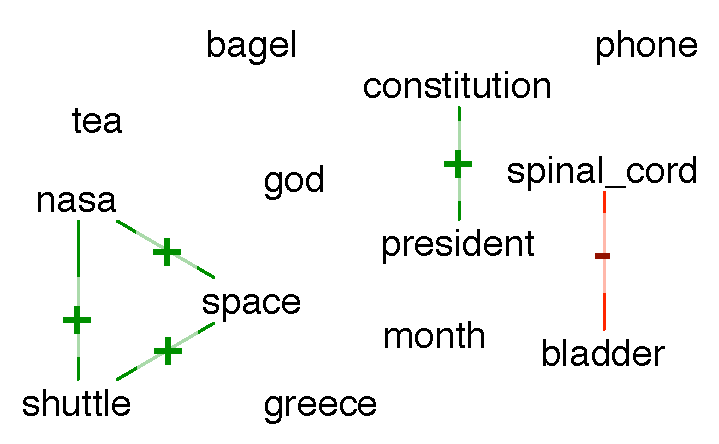
\includegraphics[width=\linewidth]{interactive_topic_models/constraints_3}     }
\end{columns}

}

\begin{frame}
  \frametitle{Adding meaning to topic models}

        \begin{itemize}
	 \item Add an additional step to model topics as a distribution over concepts

         \item We've used this formalism to build probabilistic word-sense
           disambiguation algorithms~\cite{boyd-graber-07} and multilingual models~\cite{boyd-graber-10}

         \item Others have used it to encode database constraints (e.g. cannot link and must link)~\cite{andrzejewski-09} or first order logic~\cite{andrzejewski-11}
        \end{itemize}

\end{frame}

\begin{frame}
  \frametitle{Adding meaning to topic models}
        \begin{block}{Traditional Topic Models}
                $ p(w) = \prod_d \prod_n^{N_d} \left( p(w_{d,n} | \phi_{z_{d,n}})
                  \explain{\alert<3>{topic}}{p(z_{d,n} | \theta_d)} \right) p(\theta_d | \alpha)                 \explain{\alert<2>{topic to words}}{ \prod_k^K
p(\phi_k | \eta) }$
        \end{block}

        \begin{block}{Our Model}
          \vspace{-0.8cm}
          \begin{align*}
               p(w) = \prod_d \prod_n^{N_d} & \left( p(w_{d,n} | \pi_{l_{d,n}})
                 \explain{\alert<6>{meaning and topic}} {p(l_{d,n} | \phi_{d,n} )
                   p(z_{d,n} | \theta_d)}  \right) p(\theta_d | \alpha) \\
               &  \explain{\alert<4>{topic to concept}}{\prod_k^K
                p(\phi_k | \eta)} \explain{\alert<5>{concept to word}}{\prod_c^C \left(
                  p(\pi_{k,c} | \tau) \right) }
           \end{align*}
        \end{block}


\end{frame}

\begin{frame}

        % TODO(jbg): add image
        \frametitle{Fix Ingredient \#2: Online Learning}

        \begin{itemize}
                \item Feedback shows data where you made mistakes
                \item ``Forget'' those data~\cite{yao-09}
                \item Then rerun inference, pretending you're seeing them for the first time
                \item Allows you to escape from local optima
        \end{itemize}

\end{frame}


\frame{
	\frametitle{How to incorporate feedback?}

	\begin{columns}

	\column{.5\linewidth}

		\begin{columns}

			\column{.6\linewidth}

			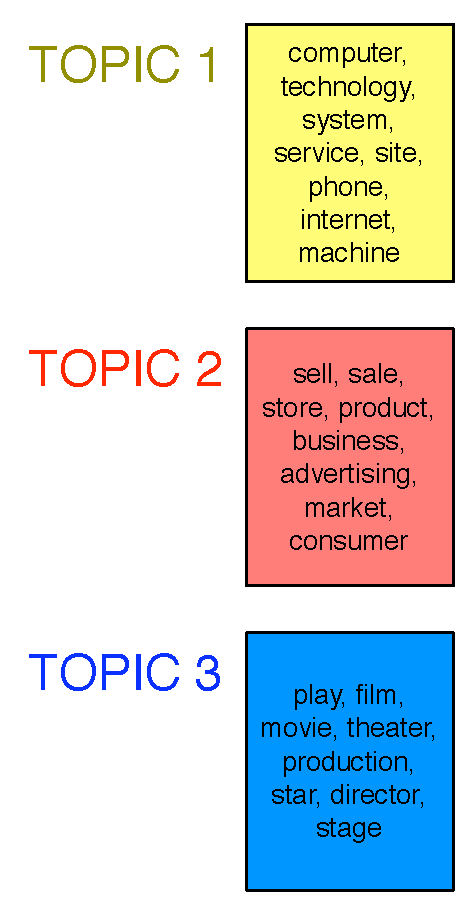
\includegraphics[width=\linewidth]{topic_models/nyt_topics}


			\column{.4\linewidth}
			\begin{center}
				\only<2->{
\includegraphics[width=.6\linewidth]{general_figures/arrow_right_down} \\}
				\only<2->{
\includegraphics[width=.6\linewidth]{general_figures/milkman_dan} \\}
				\invisible<-2>{
\includegraphics[width=.6\linewidth,angle=270]{general_figures/arrow_right_down}}
			\end{center}

		\end{columns}

	\column{.5\linewidth}

	\begin{enumerate}
		\item Fit initial topic model
			\pause
		\item Get feedback from user
			\pause
		\item Incrementally relearn model
			\begin{itemize}
                                \item Forget your mistakes
				\item Replace the model with a correlated one
				\item Continue inference
			\end{itemize}
	\end{enumerate}
\pause
Keep computation \alert<4>{fast and consistent} \cite{Hu-12a}
	\end{columns}

}

\providecommand{\tb}[1]{\parbox{0.8\linewidth}{ \tiny{ #1 }} \vspace{.2cm} }

\frame{

\vspace{-1cm}

\begin{columns}

\column{.5\linewidth}

\begin{tabular}{l*{2}{c}r}
	Topic & Before \\
\hline

\alert<2>{{\bf 1}} & \tb{ \alert<2>{election, yeltsin, russian, political, party, democratic, russia,
  president, democracy, boris, country, south, years, month, government, vote,
  since, leader, presidential, military} } \\

2 & \tb{new, york, city, state, mayor, budget, giuliani, council, cuomo, gov,
  plan, year, rudolph, dinkins, lead, need, governor, legislature, pataki,
  david} \\

3 & \tb{nuclear, arms, weapon, defense, treaty, missile, world, unite, yet,
  soviet, lead, secretary, would, control, korea, intelligence, test, nation,
  country, testing} \\

4 & \tb{president, bush, administration, clinton, american, force, reagan, war,
  unite, lead, economic, iraq, congress, america, iraqi, policy, aid,
  international, military, see} \\

& \vdots \\

\alert<2>{{\bf 20}} & \tb{\alert<2>{soviet, lead, gorbachev, union, west, mikhail, reform, change, europe,
  leaders, poland, communist, know, old, right, human, washington, western,
  bring, party} }\\

\end{tabular}

\column{.5\linewidth}

\only<3> {

	\begin{block}{Suggestion}
	\emph{boris, communist, gorbachev, mikhail, russia,
  russian, soviet, union, yeltsin }
	\end{block}

}

\only<4-> {

\begin{tabular}{l*{2}{c}r}
	Topic & After \\
\hline

\alert<5>{{\bf 1}} & \alert<5>{\tb{election, democratic, south, country, president, party, africa, lead,
  even, democracy, leader, presidential, week, politics, minister, percent,
  voter, last, month, years} } \\

\alert<6>{2} & \tb{new, york, city, state, mayor, budget, council, giuliani, gov, cuomo,
  year, rudolph, dinkins, legislature, plan, david, governor, pataki, need, cut}
\\

\alert<6>{3} & \tb{nuclear, arms, weapon, treaty, defense, war, missile, may, come, test,
  american, world, would, need, lead, get, join, yet, clinton, nation} \\

\alert<6>{4} & \tb{president, administration, bush, clinton, war, unite, force, reagan,
  american, america, make, nation, military, iraq, iraqi, troops, international,
  country, yesterday, plan} \\

   & \vdots \\

\alert<4>{ {\bf 20} } & \alert<4> {\tb{soviet, union, economic, reform, yeltsin, russian, lead, russia,
  gorbachev, leaders, west, president, boris, moscow, europe, poland, mikhail,
  communist, power, relations} } \\

\end{tabular}

}

\end{columns}

}


\providecommand{\blue}[1]{{\color{blue}{#1}}}
\providecommand{\red}[1]{{\color{red}{#1}}}
\providecommand{\green}[1]{{\color{green}{#1}}}

\begin{frame}

\frametitle{Example: Negative Constraint}

\begin{columns}

\column{.4\linewidth}

\begin{tabular}{l*{2}{c}r}
	Topic & Words \\
\hline

{\bf 318} & \tb{\red{bladder}, sci, \blue{spinal\_cord}, \blue{spinal\_cord\_injury}, \blue{spinal}, \red{urinary}, \red{urinary\_tract}, \red{urothelial},\blue{injury}, \blue{motor}, \blue{recovery}, \blue{reflex}, \blue{cervical}, \red{urothelium}, \blue{functional\_recovery}} \\

\end{tabular}

\column{.1\linewidth}

\column{.4\linewidth}

\only<3->{
\begin{tabular}{l*{2}{c}r}
	Topic & Words \\
\hline

{\bf 318} & \tb{sci, \blue{spinal\_cord}, \blue{spinal\_cord\_injury}, \blue{spinal}, \blue{injury}, \blue{recovery}, \blue{motor}, \blue{reflex}, \red{urothelial}, \green{injured}, \blue{functional\_recovery}, \green{plasticity}, \green{locomotor}, \blue{cervical}, \green{locomotion}}\\

\end{tabular}
}

\end{columns}

\only<2->{
\begin{block}{Negative Constraint}
  spinal\_cord, bladder
\end{block}

}

\end{frame}




\begin{frame}

        \frametitle{Experiments}

\begin{columns}

\column{.5\linewidth}

  \begin{itemize}
   \item Simulating users through classifying social media
     \begin{itemize}
       \item Investigating different learning strategies
       \item How much to forget
     \end{itemize}
   \end{itemize}

\column{.5\linewidth}

\begin{center}
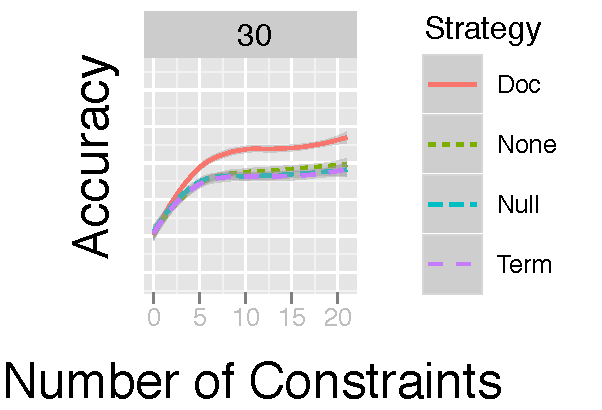
\includegraphics[width=\linewidth]{interactive_topic_models/ablation_30_topics}
\end{center}

\end{columns}

\begin{itemize}
    \item User study: mechanical Turk
      \begin{itemize}
        \item We can't do everything users want: proper names, mac vs. pc
        \item Users are senstive to polysemy (``msg'': food or e-mail)
      \end{itemize}
    \item User study: exploring congressional debates
      \begin{itemize}
        \item Collaboration with social scientists
        \item Interactivity makes people use topic models more
       \end{itemize}
  \end{itemize}


\end{frame}
